% !TEX TS-program = xelatex
%
\documentclass{beamer}

\usetheme{metropolis}

\usepackage{fontspec}
\defaultfontfeatures{Ligatures=TeX}

\usefonttheme{professionalfonts}
\usepackage[familydefault,light]{Chivo}

\usepackage{setspace}

\usepackage{tkz-graph}
\tikzset{vertex/.style = {shape=circle,draw,minimum size=1}}
\tikzset{edge/.style = {->,> = latex'}}

\newcommand{\highlight}[1]{{\usebeamercolor[fg]{example text}#1}}

\hypersetup
{
  pdftitle   = {Process Calculi for Concurrency},
  pdfauthor  = {Michael Kaltschmid \& Markus Reiter}
}

\title{Process Calculi}
\subtitle{for Concurrency}
\author{Michael Kaltschmid \& Markus Reiter}
\date{}

\begin{document}
  \maketitle

  \begin{frame}{Outline}
    \begin{itemize}
      \item What is a Process Calculus?
      \item µ-Calculus
      \item mCRL2
    \end{itemize}
  \end{frame}

  \begin{frame}{What is a Process Calculus?}
    \begin{itemize}
      \item approach for formally modelling concurrent systems
      \item tool for high-level description of interactions, communications and synchronizations between processes
      \item provides algebraic laws to allow analyzing and transforming process descriptions
      \item permits formal reasoning about equivalences between processes (e.g., using bisimulation)
    \end{itemize}
  \end{frame}

  \begin{frame}{Process Calculi}
    \begin{itemize}
      \item ACP
      \item CCS
      \item CSP
      \item Join-Calculus
      \item \textbf{µ-Calculus}
      \item PEPA
      \item π-Calculus
    \end{itemize}
  \end{frame}

  \begin{frame}{Syntax}
    The set of µ-calculus formulas, $\mathcal{F}$ is the smallest set containing: \\[12pt]
    \begin{itemize}
      \item $p$ and $\neg p$ for all propositions $p \in Prop$ \\
      \item $X$ for all variables $X \in Var$ \\
      \item $\phi \lor \psi$ and $\phi \land \psi$, if $\phi$, $\psi$ are formulas in $\mathcal{F}$
      \item ($a$)$\phi$ and [$a$]$\psi$, if $a \in Act$ is an action and $\phi$ is a formual in  $\mathcal{F}$
      \item $\mu X. \phi$ and $v X. \phi$, if $X \in Var$ is a variable and $\phi \in \mathcal{F}$ is a formula.
    \end{itemize}
  \end{frame}

  \begin{frame}{Labelled Trainsiton Systems}
    Given a labelled transition system $(S, R, V)$: \\[12pt]
    \begin{itemize}
      \item $S$ is a set of states \\
      \item $R$ maps to each label $a$ a binary relation on $S$ \\
      \item $V:P\rightarrow 2^{S}$, maps to each proposition $p \in P$ the set of states where the proposition is true
    \end{itemize}
  \end{frame}


  \begin{frame}{Diamond \& Box Modalities}
    \resizebox{\textwidth}{!}{
      \renewcommand{\arraystretch}{2}
      \begin{tabular}{l c c c c}
        &

        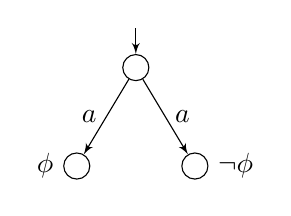
\begin{tikzpicture}
          \node[vertex] (a) at (0.75, 1.25) {};
          \node[vertex] [label=left:{$\phi$}] (b) at (0, 0) {};
          \node[vertex] [label=right:{$\neg\phi$}] (c) at (1.5, 0) {};

          \draw[edge] (.75, 1.75) to (a);
          \draw[edge] (a) to node [left] {$a$} (b);
          \draw[edge] (a) to node [right] {$a$} (c);
        \end{tikzpicture}

        &

        \begin{tikzpicture}
          \node[vertex] (a) at (0, 1.25) {};
          \node at (0, -0.175) {};

          \draw[edge] (0, 1.75) to (a);
        \end{tikzpicture}

        &

        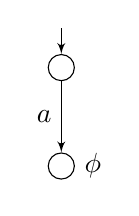
\begin{tikzpicture}
          \node[vertex] (a) at (0, 1.25) {};
          \node[vertex] [label=right:{$\phi$}] (b) at (0, 0) {};

          \draw[edge] (0, 1.75) to (a);
          \draw[edge] (a) to node [left] {$a$} (b);
        \end{tikzpicture}

        &

        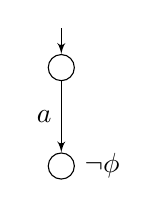
\begin{tikzpicture}
          \node[vertex] (a) at (0, 1.25) {};
          \node[vertex] [label=right:{$\neg\phi$}] (b) at (0, 0) {};

          \draw[edge] (0, 1.75) to (a);
          \draw[edge] (a) to node [left] {$a$} (b);
        \end{tikzpicture}

        \\

        $\langle{}a\rangle{}\phi$ & \highlight{valid} & \alert{invalid}   & \highlight{valid} & \alert{invalid} \\

        $[a]\phi$                 & \alert{invalid}   & \highlight{valid} & \highlight{valid} & \alert{invalid} \\
      \end{tabular}
    }
  \end{frame}

  \begin{frame}{Regular Formulae}
    \begin{itemize}
      \item allow more than a single action in a modality
      \item useful for expressing that after two or more \\
            arbitrary actions, a specific action must happen
      \item based on action formulae
    \end{itemize}

    \begin{exampleblock}{A more concrete example:}
      After two \textit{\textbf{receive}} actions, a \textit{\textbf{send}} action must follow.
    \end{exampleblock}
  \end{frame}

  \begin{frame}{Action Formulae}
    An action formula $af$ defines a set of multi-actions.

    \begin{align*}
      af ::= \alpha\ |\ true\ |\ false\ |\ \overline{af}\ |\ af\ \cap\ af\ |\ af\ \cup\ af
    \end{align*}

    \begin{itemize}
      \item $\alpha$ represents the set with exactly the multi-action $\alpha$.
      \item $true$ is the set of all multi-actions.
      \item $false$ is the empty set.
      \item $\overline{af}$ denotes the complement of the set $af$.
      \item $\cup$ and $\cap$ denote union and intersection, respectively.
    \end{itemize}
  \end{frame}

  \begin{frame}{Action Formulae}
    $af$ being a set of multi-actions, modalities with action formulae are defined like this:

    \begin{align*}
      \langle{af}\rangle\phi = \bigvee_{\alpha \in af} \langle\alpha\rangle\phi
      \qquad\qquad
      [af]\phi = \bigwedge_{\alpha \in af} [\alpha]\phi
    \end{align*}

    \begin{exampleblock}{Example}
      \begin{itemize}
        \item $\langle\overline{a}\rangle\langle{b \cup c}\rangle{true}$ means an action other than $a$ can be done, followed by either $b$ or $c$.
        \item $[\overline{a}]false$ says that only an $a$ action is allowed.
      \end{itemize}
    \end{exampleblock}
  \end{frame}

  \begin{frame}{Regular Formulae}
    Regular formulae extend action formulae, allowing sequences of actions in modalities.

    \begin{align*}
      \highlight{
        R ::= \epsilon\ |\ af\ |\ R\cdot{R}\ |\ R+R\ |\ R^*\ |\ R^+
      }
    \end{align*}

    \begin{itemize}
      \item $\epsilon$ is the empty sequence of actions.
      \item $R_1\cdot{R_2}$ represents the concatenation of $R_1$ and $R_2$.
      \item $R_1+R_2$ denotes the union of  $R_1$ and $R_2$.
      \item $R^*$ denotes zero ore more repetitions.
      \item $R^+$ denotes one ore more repetitions.
    \end{itemize}
  \end{frame}

  \begin{frame}[t]{Regular Formulae}
    \begin{exampleblock}{Examples}
      \begin{itemize}
        \item $[\epsilon]\phi = \langle\epsilon\rangle\phi = \phi$, so one can always perform no action, and remain in the same state.
        \item $\langle{a}\cdot{b}\cdot{c}\rangle{true}$ is the same as $\langle{a}\rangle\langle{b}\rangle\langle{c}\rangle{true}$.
        \item $[a\cdot{b} + c\cdot{d}]false$ means that neither the sequence $a\cdot{b}$ nor $c\cdot{d}$ is possible.
        \item $\langle{a^*}\rangle{true}$ expresses that any sequence of $a$ actions is possible.
        \item $[a^+]\phi$ says that $\phi$ must hold in any state reachable by one or more $a$ actions.
      \end{itemize}
    \end{exampleblock}
  \end{frame}
\end{document}
